% Options for packages loaded elsewhere
% Options for packages loaded elsewhere
\PassOptionsToPackage{unicode}{hyperref}
\PassOptionsToPackage{hyphens}{url}
%
\documentclass[
  14pt,
  ignorenonframetext,
  aspectratio=169,
]{beamer}
\newif\ifbibliography
\usepackage{pgfpages}
\setbeamertemplate{caption}[numbered]
\setbeamertemplate{caption label separator}{: }
\setbeamercolor{caption name}{fg=normal text.fg}
\beamertemplatenavigationsymbolsempty
% remove section numbering
\setbeamertemplate{part page}{
  \centering
  \begin{beamercolorbox}[sep=16pt,center]{part title}
    \usebeamerfont{part title}\insertpart\par
  \end{beamercolorbox}
}
\setbeamertemplate{section page}{
  \centering
  \begin{beamercolorbox}[sep=12pt,center]{section title}
    \usebeamerfont{section title}\insertsection\par
  \end{beamercolorbox}
}
\setbeamertemplate{subsection page}{
  \centering
  \begin{beamercolorbox}[sep=8pt,center]{subsection title}
    \usebeamerfont{subsection title}\insertsubsection\par
  \end{beamercolorbox}
}
% Prevent slide breaks in the middle of a paragraph
\widowpenalties 1 10000
\raggedbottom
\usepackage{iftex}
\ifPDFTeX
  \usepackage[T1]{fontenc}
  \usepackage[utf8]{inputenc}
  \usepackage{textcomp} % provide euro and other symbols
\else % if luatex or xetex
  \usepackage{unicode-math} % this also loads fontspec
  \defaultfontfeatures{Scale=MatchLowercase}
  \defaultfontfeatures[\rmfamily]{Ligatures=TeX,Scale=1}
\fi
\usepackage{lmodern}

\usetheme[]{monash}
\ifPDFTeX\else
  % xetex/luatex font selection
\fi
% Use upquote if available, for straight quotes in verbatim environments
\IfFileExists{upquote.sty}{\usepackage{upquote}}{}
\IfFileExists{microtype.sty}{% use microtype if available
  \usepackage[]{microtype}
  \UseMicrotypeSet[protrusion]{basicmath} % disable protrusion for tt fonts
}{}
\makeatletter
\@ifundefined{KOMAClassName}{% if non-KOMA class
  \IfFileExists{parskip.sty}{%
    \usepackage{parskip}
  }{% else
    \setlength{\parindent}{0pt}
    \setlength{\parskip}{6pt plus 2pt minus 1pt}}
}{% if KOMA class
  \KOMAoptions{parskip=half}}
\makeatother

\usepackage{color}
\usepackage{fancyvrb}
\newcommand{\VerbBar}{|}
\newcommand{\VERB}{\Verb[commandchars=\\\{\}]}
\DefineVerbatimEnvironment{Highlighting}{Verbatim}{commandchars=\\\{\}}
% Add ',fontsize=\small' for more characters per line
\usepackage{framed}
\definecolor{shadecolor}{RGB}{248,248,248}
\newenvironment{Shaded}{\begin{snugshade}}{\end{snugshade}}
\newcommand{\AlertTok}[1]{\textcolor[rgb]{0.94,0.16,0.16}{#1}}
\newcommand{\AnnotationTok}[1]{\textcolor[rgb]{0.56,0.35,0.01}{\textbf{\textit{#1}}}}
\newcommand{\AttributeTok}[1]{\textcolor[rgb]{0.13,0.29,0.53}{#1}}
\newcommand{\BaseNTok}[1]{\textcolor[rgb]{0.00,0.00,0.81}{#1}}
\newcommand{\BuiltInTok}[1]{#1}
\newcommand{\CharTok}[1]{\textcolor[rgb]{0.31,0.60,0.02}{#1}}
\newcommand{\CommentTok}[1]{\textcolor[rgb]{0.56,0.35,0.01}{\textit{#1}}}
\newcommand{\CommentVarTok}[1]{\textcolor[rgb]{0.56,0.35,0.01}{\textbf{\textit{#1}}}}
\newcommand{\ConstantTok}[1]{\textcolor[rgb]{0.56,0.35,0.01}{#1}}
\newcommand{\ControlFlowTok}[1]{\textcolor[rgb]{0.13,0.29,0.53}{\textbf{#1}}}
\newcommand{\DataTypeTok}[1]{\textcolor[rgb]{0.13,0.29,0.53}{#1}}
\newcommand{\DecValTok}[1]{\textcolor[rgb]{0.00,0.00,0.81}{#1}}
\newcommand{\DocumentationTok}[1]{\textcolor[rgb]{0.56,0.35,0.01}{\textbf{\textit{#1}}}}
\newcommand{\ErrorTok}[1]{\textcolor[rgb]{0.64,0.00,0.00}{\textbf{#1}}}
\newcommand{\ExtensionTok}[1]{#1}
\newcommand{\FloatTok}[1]{\textcolor[rgb]{0.00,0.00,0.81}{#1}}
\newcommand{\FunctionTok}[1]{\textcolor[rgb]{0.13,0.29,0.53}{\textbf{#1}}}
\newcommand{\ImportTok}[1]{#1}
\newcommand{\InformationTok}[1]{\textcolor[rgb]{0.56,0.35,0.01}{\textbf{\textit{#1}}}}
\newcommand{\KeywordTok}[1]{\textcolor[rgb]{0.13,0.29,0.53}{\textbf{#1}}}
\newcommand{\NormalTok}[1]{#1}
\newcommand{\OperatorTok}[1]{\textcolor[rgb]{0.81,0.36,0.00}{\textbf{#1}}}
\newcommand{\OtherTok}[1]{\textcolor[rgb]{0.56,0.35,0.01}{#1}}
\newcommand{\PreprocessorTok}[1]{\textcolor[rgb]{0.56,0.35,0.01}{\textit{#1}}}
\newcommand{\RegionMarkerTok}[1]{#1}
\newcommand{\SpecialCharTok}[1]{\textcolor[rgb]{0.81,0.36,0.00}{\textbf{#1}}}
\newcommand{\SpecialStringTok}[1]{\textcolor[rgb]{0.31,0.60,0.02}{#1}}
\newcommand{\StringTok}[1]{\textcolor[rgb]{0.31,0.60,0.02}{#1}}
\newcommand{\VariableTok}[1]{\textcolor[rgb]{0.00,0.00,0.00}{#1}}
\newcommand{\VerbatimStringTok}[1]{\textcolor[rgb]{0.31,0.60,0.02}{#1}}
\newcommand{\WarningTok}[1]{\textcolor[rgb]{0.56,0.35,0.01}{\textbf{\textit{#1}}}}

\usepackage{longtable,booktabs,array}
\newcounter{none} % for unnumbered tables
\usepackage{calc} % for calculating minipage widths
\usepackage{caption}
% Make caption package work with longtable
\makeatletter
\def\fnum@table{\tablename~\thetable}
\makeatother
\usepackage{graphicx}
\makeatletter
\newsavebox\pandoc@box
\newcommand*\pandocbounded[1]{% scales image to fit in text height/width
  \sbox\pandoc@box{#1}%
  \Gscale@div\@tempa{\textheight}{\dimexpr\ht\pandoc@box+\dp\pandoc@box\relax}%
  \Gscale@div\@tempb{\linewidth}{\wd\pandoc@box}%
  \ifdim\@tempb\p@<\@tempa\p@\let\@tempa\@tempb\fi% select the smaller of both
  \ifdim\@tempa\p@<\p@\scalebox{\@tempa}{\usebox\pandoc@box}%
  \else\usebox{\pandoc@box}%
  \fi%
}
% Set default figure placement to htbp
\def\fps@figure{htbp}
\makeatother





\setlength{\emergencystretch}{3em} % prevent overfull lines

\providecommand{\tightlist}{%
  \setlength{\itemsep}{0pt}\setlength{\parskip}{0pt}}



 


% Colors
\definecolor{shadecolor}{RGB}{225,225,225}
\setbeamercolor{description item}{fg=Orange}
\definecolor{MonashBlue}{RGB}{66,109,152}
\definecolor{burntorange}{rgb}{0.8, 0.33, 0.0}

% Packages
\usepackage{amsmath, bm, amssymb, amsthm, mathrsfs,pifont}
\usepackage{url}
\usepackage{multirow, booktabs, float, textcmds, siunitx}
\usepackage{bm,booktabs,animate,ragged2e,multicol,microtype,hyperref}
\usepackage{fontawesome5}

% Figures
\graphicspath{{figs/}}

% Fonts
\fontsize{13}{15}\sf
\setbeamerfont{title}{series=\bfseries,parent=structure,size=\fontsize{24}{24}}
\ifcsname Shaded\endcsname
  \definecolor{shadecolor}{RGB}{225,225,225}
  \renewenvironment{Shaded}{\vspace*{0.15cm}\color{black}\fontsize{10}{10}\sf\begin{snugshade}\color{black}}{\end{snugshade}}
\fi

% gt dependencies
\usepackage{longtable,caption,setspace}
\captionsetup{font={small,stretch=0.80}}

% My definitions

\def\E{\text{E}}
\def\V{\text{Var}}
\def\up#1{\raisebox{-0.3cm}{#1}}
\def\pred#1#2#3{\hat{#1}_{#2|#3}}
\def\damped{$_\text{d}$}
\def\h+{h_{m}^{+}}
\def\str#1{\rlap{#1}\textcolor{red}{\rule{1cm}{0.1cm}}}

\def\st#1{\rlap{#1}\textcolor{red}{\rule{1cm}{0.1cm}}}
\def\bY{\bm{y}}
\def\by{\bm{y}}
\def\bS{\bm{S}}
\def\bI{\text{\rm\textbf{I}}}
\def\bbeta{\bm{\beta}}
\def\bSigma{\bm{\Sigma}}
\def\bW{\bm{\Sigma}}
\def\Var{\text{Var}}
\def\var{\text{Var}}
\def\bOmega{\bm{\Omega}}
\def\bLambda{\bm{\Lambda}}
\let\mc\multicolumn
\def\hl{\color[RGB]{230, 172, 0}}

\def\forecast{\begin{alertblock}{}\fontsize{10}{11}\sf
 A forecast is an estimate of the probability distribution of a variable to be observed in the future.
\end{alertblock}}

\def\simfutures{\begin{textblock}{2.9}(12.8,7.7)
\begin{block}{}\fontsize{10}{11}\sf
Simulated futures from an ETS model
\end{block}\end{textblock}}

\setbeamertemplate{title page}
{\placefig{0}{-0.5}{width=1.01\paperwidth,height=1.45\paperheight}{africa1.jpg}
\begin{textblock}{8.5}(.5,0.2)
  \raggedright\fontsize{20}{20}\selectfont\bfseries\sffamily\textcolor{white}{\inserttitle}\\[0.2cm]
  \fontsize{12}{12}\selectfont\bfseries\sffamily\textcolor{white}{\insertsubtitle}
  \end{textblock}
\placefig{.5}{6.2}{width=2.4cm}{tsibble.png}
\placefig{2.9}{6.2}{width=2.4cm}{feasts.png}
\placefig{5.3}{6.2}{width=2.4cm}{fable.png}
\begin{textblock}{7.5}(10.6,-.1)
  {\fontsize{9}{9}\sf\color{white}https://workshop.f4sg.org/africast/}
\end{textblock}
}

% Tikz plots
\usepackage{tikz}
\usetikzlibrary{trees,shapes,arrows,matrix,shadows,positioning,calc}
\tikzstyle{decision} = [diamond, draw, fill=blue!20,
    text width=4.5em, text badly centered, node distance=4cm, inner sep=0pt]
\tikzstyle{block} = [rectangle, draw, fill=blue!20,
    text width=5cm, text centered, rounded corners, minimum height=4em]
\tikzstyle{line} = [draw, thick, -latex']
\tikzstyle{cloud} = [draw, ellipse,fill=red!20, node distance=3cm,
    minimum height=2em, text centered]
\tikzstyle{connector} = [->,thick]

\tikzset{
  basic/.style  = {draw, text width=2cm, font=\sffamily, rectangle},
  root/.style   = {basic, text width=3cm, rounded corners=2pt, thin, align=center, fill=red!30},
  level 2a/.style = {basic, rounded corners=2pt, thin,align=center, fill=blue!50, text width=7em},
  level 2b/.style = {basic, rounded corners=2pt, thin,align=center, fill=green!50, text width=7em},
  level 3a/.style = {basic, rounded corners=2pt, thin, align=center, fill=blue!30, text width=4em},
  level 3b/.style = {basic, rounded corners=2pt, thin, align=center, fill=green!30, text width=4em},
  level 4a/.style = {basic, rounded corners=2pt, thin, align=left, fill=blue!10, text width=3.5em},
  level 4b/.style = {basic, rounded corners=2pt, thin, align=left, fill=green!10, text width=3.5em}
}

% % BIBLIOGRAPHIES
% \usepackage[style=authoryear,bibencoding=utf8,minnames=1,maxnames=4, maxbibnames=99,natbib=true,dashed=false,terseinits=true,giveninits=true,uniquename=false,uniquelist=false,labeldate=true,doi=false, isbn=false, natbib=true,backend=biber]{biblatex}

% \DeclareFieldFormat{url}{\url{#1}}
% \DeclareFieldFormat[article]{pages}{#1}
% \DeclareFieldFormat[inproceedings]{pages}{\lowercase{pp.}#1}
% \DeclareFieldFormat[incollection]{pages}{\lowercase{pp.}#1}
% \DeclareFieldFormat[article]{volume}{\mkbibbold{#1}}
% \DeclareFieldFormat[article]{number}{\mkbibparens{#1}}
% \DeclareFieldFormat[article]{title}{\MakeCapital{#1}}
% \DeclareFieldFormat[article]{url}{}
% \DeclareFieldFormat[Techreport]{Url}{}
% \DeclareFieldFormat[book]{url}{}
% \DeclareFieldFormat[inbook]{url}{}
% \DeclareFieldFormat[incollection]{url}{}
% \DeclareFieldFormat[inproceedings]{url}{}
% \DeclareFieldFormat[inproceedings]{title}{#1}
% \DeclareFieldFormat{shorthandwidth}{#1}
% %\DeclareFieldFormat{extrayear}{}
% % No dot before number of articles
% \usepackage{xpatch}
% \xpatchbibmacro{volume+number+eid}{\setunit*{\adddot}}{}{}{}
% % Remove In: for an article.
% \renewbibmacro{in:}{%
%   \ifentrytype{article}{}{%
%   \printtext{\bibstring{in}\intitlepunct}}}

% \AtEveryBibitem{\clearfield{month}}
% \AtEveryCitekey{\clearfield{month}}
% \AtBeginBibliography{\fontsize{11}{11}\sf}
\setbeamertemplate{frametitle continuation}{}
\makeatletter
\@ifpackageloaded{caption}{}{\usepackage{caption}}
\AtBeginDocument{%
\ifdefined\contentsname
  \renewcommand*\contentsname{Table of contents}
\else
  \newcommand\contentsname{Table of contents}
\fi
\ifdefined\listfigurename
  \renewcommand*\listfigurename{List of Figures}
\else
  \newcommand\listfigurename{List of Figures}
\fi
\ifdefined\listtablename
  \renewcommand*\listtablename{List of Tables}
\else
  \newcommand\listtablename{List of Tables}
\fi
\ifdefined\figurename
  \renewcommand*\figurename{Figure}
\else
  \newcommand\figurename{Figure}
\fi
\ifdefined\tablename
  \renewcommand*\tablename{Table}
\else
  \newcommand\tablename{Table}
\fi
}
\@ifpackageloaded{float}{}{\usepackage{float}}
\floatstyle{ruled}
\@ifundefined{c@chapter}{\newfloat{codelisting}{h}{lop}}{\newfloat{codelisting}{h}{lop}[chapter]}
\floatname{codelisting}{Listing}
\newcommand*\listoflistings{\listof{codelisting}{List of Listings}}
\makeatother
\makeatletter
\makeatother
\makeatletter
\@ifpackageloaded{caption}{}{\usepackage{caption}}
\@ifpackageloaded{subcaption}{}{\usepackage{subcaption}}
\makeatother

\usepackage{bookmark}
\IfFileExists{xurl.sty}{\usepackage{xurl}}{} % add URL line breaks if available
\urlstyle{same}
% fallback for those not using the hyperref driver hyperxmp:
\makeatletter
\@ifundefined{xmpquote}{\newcommand{\xmpquote}[1]{#1}}{}
\makeatother
\hypersetup{
  pdftitle={Africast-Time Series Analysis \& Forecasting Using R},
  hidelinks,
  pdfcreator={LaTeX via pandoc}}


\title{\texorpdfstring{Africast-Time Series Analysis \& Forecasting
Using R}{Africast-Time Series Analysis \& Forecasting Using R}}
\subtitle{\texorpdfstring{7. Exponential
smoothing}{7. Exponential smoothing}}
\author{}
\date{6 October 2026}

\begin{document}
\frame{\titlepage}


\begin{frame}{Outline}
\protect\phantomsection\label{outline}
\vspace*{0.7cm}\tableofcontents
\end{frame}

\section{Exponential smoothing}\label{exponential-smoothing}

\begin{frame}{From simple methods to Exponential Smoothing}
\protect\phantomsection\label{from-simple-methods-to-exponential-smoothing}
\begin{itemize}
\tightlist
\item
  Naive method: Use only the last observation
\item
  Average method: Use all observations
\item
  Want something in between naive and average methods.
\item
  Most recent data should have more weight.
\item
  This is exactly the concept behind exponential smoothing
\end{itemize}
\end{frame}

\begin{frame}{Pegel's classification}
\protect\phantomsection\label{pegels-classification}
\begin{center}
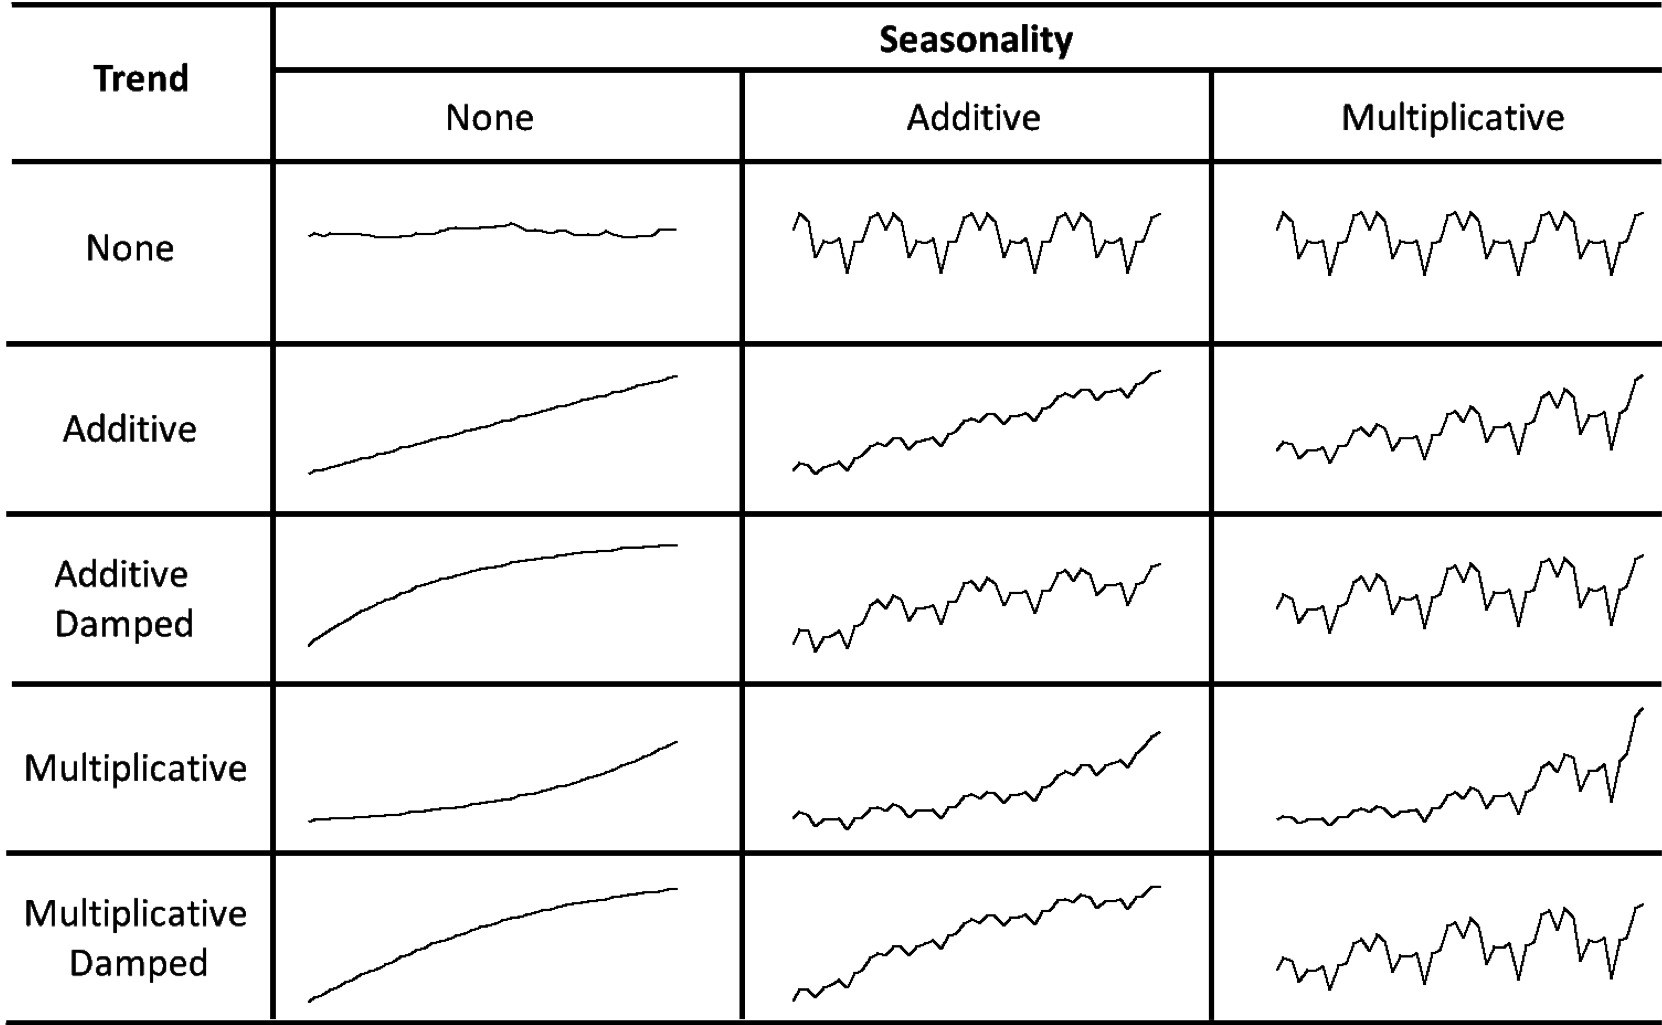
\includegraphics[width=0.9\linewidth,height=\textheight,keepaspectratio]{figs/pegel1.png}
\end{center}
\end{frame}

\begin{frame}{Historical perspective}
\protect\phantomsection\label{historical-perspective}
\begin{itemize}
\tightlist
\item
  Developed in the 1950s and 1960s as methods (algorithms) to produce
  point forecasts.
\item
  Combine a ``level'', ``trend'' (slope) and ``seasonal'' component to
  describe a time series.
\item
  The rate of change of the components are controlled by ``smoothing
  parameters'': \(\alpha\), \(\beta\) and \(\gamma\) respectively.
\item
  Need to choose best values for the smoothing parameters (and initial
  states).
\item
  Equivalent ETS state space models developed in the 1990s and 2000s.
\end{itemize}
\end{frame}

\begin{frame}{A model for levels, trends, and seasonalities}
\protect\phantomsection\label{a-model-for-levels-trends-and-seasonalities}
\fontsize{13}{13}\sf

We want a model that captures the level (\(\ell_t\)), trend (\(b_t\))
and seasonality (\(s_t\)).\vspace*{-0.1cm}

\alert{How do we combine these elements?}

\pause

\begin{block}{Additively?}
$y_t = \ell_{t-1} + b_{t-1} + s_{t-m} + \varepsilon_t$
\end{block}\pause
\begin{block}{Multiplicatively?}
$y_t = \ell_{t-1}b_{t-1}s_{t-m}(1 + \varepsilon_t)$
\end{block}\pause
\begin{block}{Perhaps a mix of both?}
$y_t = (\ell_{t-1} + b_{t-1}) s_{t-m} + \varepsilon_t$
\end{block}\pause\vspace*{-0.1cm}

\alert{How do the level, trend and seasonal components evolve over time?}
\end{frame}

\begin{frame}[fragile]{ETS models}
\protect\phantomsection\label{ets-models}
\begin{block}{}
\hspace*{-0.25cm}\begin{tabular}{l@{}p{2.3cm}@{}c@{}l}
\structure{General n\rlap{otation}}
    &       & ~E T S~  & ~:\hspace*{0.3cm}\textbf{E}xponen\textbf{T}ial \textbf{S}moothing               \\ [-0.2cm]
    & \hfill{$\nearrow$\hspace*{-0.1cm}}        & {$\uparrow$} & {\hspace*{-0.2cm}$\nwarrow$} \\
    & \hfill{\textbf{E}rror\hspace*{0.2cm}} & {\textbf{T}rend}      & {\hspace*{0.2cm}\textbf{S}eason}
\end{tabular}
\end{block}

\alert{\textbf{E}rror:} Additive (\texttt{"A"}) or multiplicative
(\texttt{"M"}) \pause

\alert{\textbf{T}rend:} None (\texttt{"N"}), additive (\texttt{"A"}),
multiplicative (\texttt{"M"}), or damped (\texttt{"Ad"} or
\texttt{"Md"}). \pause

\alert{\textbf{S}easonality:} None (\texttt{"N"}), additive
(\texttt{"A"}) or multiplicative (\texttt{"M"})
\end{frame}

\begin{frame}{ETS(A,N,N): SES with additive errors}
\protect\phantomsection\label{etsann-ses-with-additive-errors}
\begin{block}{}\vspace*{-0.7cm}
\begin{align*}
\text{Forecast equation}&& \hat{y}_{T+h|T} &= \ell_T \\
\text{Measurement equation}&& y_t &= \ell_{t-1} + \varepsilon_t\\
\text{State equation}&& \ell_t&=\ell_{t-1}+\alpha \varepsilon_t
\end{align*}
\end{block}\vspace*{-0.4cm}

where \(\varepsilon_t\sim\text{NID}(0,\sigma^2)\).\pause

\begin{itemize}
\tightlist
\item
  ``innovations'' or ``single source of error'' because equations have
  the same error process, \(\varepsilon_t\).
\item
  Measurement equation: relationship between observations and states.
\item
  Transition/state equation(s): evolution of state(s) over time.
\end{itemize}

\vspace*{10cm}
\end{frame}

\begin{frame}{ETS(M,N,N): SES with multiplicative errors}
\protect\phantomsection\label{etsmnn-ses-with-multiplicative-errors}
\begin{block}{}\vspace*{-0.7cm}
\begin{align*}
\text{Forecast equation}&& \hat{y}_{T+h|T} &= \ell_T \\
\text{Measurement equation}&& y_t &= \ell_{t-1}(1 + \varepsilon_t)\\
\text{State equation}&& \ell_t&=\ell_{t-1} (1+\alpha\varepsilon_t)
\end{align*}
\end{block}\vspace*{-0.4cm}

where \(\varepsilon_t\sim\text{NID}(0,\sigma^2)\).\pause

\begin{itemize}
\tightlist
\item
  Models with additive and multiplicative errors with the same
  parameters generate the same point forecasts but different prediction
  intervals.
\end{itemize}

\vspace*{10cm}
\end{frame}

\section{Trend methods}\label{trend-methods}

\begin{frame}{Holt's linear trend}
\protect\phantomsection\label{holts-linear-trend}
\fontsize{13}{15}\sf

\begin{block}{Additive errors: ETS(A,A,N)}\vspace*{-0.7cm}
\begin{align*}
\text{Forecast equation}&& \hat{y}_{T+h|T} &= \ell_T + hb_T\\
\text{Measurement equation}&& y_t &= \ell_{t-1}+b_{t-1}+\varepsilon_t\\
\text{State equations}&&       \ell_t&=\ell_{t-1}+b_{t-1}+\alpha \varepsilon_t\\
&&      b_t&=b_{t-1}+\beta \varepsilon_t
\end{align*}
\end{block}
\pause

\begin{block}{Multiplicative errors: ETS(M,A,N)}\vspace*{-0.7cm}
\begin{align*}
\text{Forecast equation}&& \hat{y}_{T+h|T} &= \ell_T + hb_T\\
\text{Measurement equation}&& y_t &= (\ell_{t-1}+b_{t-1})(1+\varepsilon_t)\\
\text{State equations}&&       \ell_t&=(\ell_{t-1}+b_{t-1})(1+\alpha \varepsilon_t)\\
&&      b_t&=b_{t-1}+\beta (\ell_{t-1}+b_{t-1})\varepsilon_t
\end{align*}
\end{block}
\end{frame}

\begin{frame}[fragile]{Example: Australian population}
\protect\phantomsection\label{example-australian-population}
\fontsize{9}{9}\sf

\begin{Shaded}
\begin{Highlighting}[]
\NormalTok{aus\_economy }\OtherTok{\textless{}{-}}\NormalTok{ global\_economy }\SpecialCharTok{|\textgreater{}}
  \FunctionTok{filter}\NormalTok{(Country }\SpecialCharTok{==} \StringTok{"Australia"}\NormalTok{) }\SpecialCharTok{|\textgreater{}}
  \FunctionTok{mutate}\NormalTok{(}\AttributeTok{Pop =}\NormalTok{ Population }\SpecialCharTok{/} \FloatTok{1e6}\NormalTok{)}
\NormalTok{fit }\OtherTok{\textless{}{-}}\NormalTok{ aus\_economy }\SpecialCharTok{|\textgreater{}} \FunctionTok{model}\NormalTok{(}\AttributeTok{AAN =} \FunctionTok{ETS}\NormalTok{(Pop))}
\FunctionTok{report}\NormalTok{(fit)}
\end{Highlighting}
\end{Shaded}

\begin{verbatim}
Series: Pop 
Model: ETS(A,A,N) 
  Smoothing parameters:
    alpha = 1 
    beta  = 0.327 

  Initial states:
 l[0]  b[0]
 10.1 0.222

  sigma^2:  0.0041

  AIC  AICc   BIC 
-77.0 -75.8 -66.7 
\end{verbatim}
\end{frame}

\begin{frame}[fragile]{Example: Australian population}
\protect\phantomsection\label{example-australian-population-1}
\fontsize{10}{11}\sf

\begin{Shaded}
\begin{Highlighting}[]
\FunctionTok{components}\NormalTok{(fit)}
\end{Highlighting}
\end{Shaded}

\begin{verbatim}
# A dable: 59 x 7 [1Y]
# Key:     Country, .model [1]
# :        Pop = lag(level, 1) + lag(slope, 1) + remainder
   Country   .model  Year   Pop level slope remainder
   <fct>     <chr>  <dbl> <dbl> <dbl> <dbl>     <dbl>
 1 Australia AAN     1959  NA    10.1 0.222 NA       
 2 Australia AAN     1960  10.3  10.3 0.222 -0.000145
 3 Australia AAN     1961  10.5  10.5 0.217 -0.0159  
 4 Australia AAN     1962  10.7  10.7 0.231  0.0418  
 5 Australia AAN     1963  11.0  11.0 0.223 -0.0229  
 6 Australia AAN     1964  11.2  11.2 0.221 -0.00641 
 7 Australia AAN     1965  11.4  11.4 0.221 -0.000314
 8 Australia AAN     1966  11.7  11.7 0.235  0.0418  
 9 Australia AAN     1967  11.8  11.8 0.206 -0.0869  
10 Australia AAN     1968  12.0  12.0 0.208  0.00350 
# i 49 more rows
\end{verbatim}
\end{frame}

\begin{frame}[fragile]{Example: Australian population}
\protect\phantomsection\label{example-australian-population-2}
\fontsize{10}{11}\sf

\begin{Shaded}
\begin{Highlighting}[]
\FunctionTok{components}\NormalTok{(fit) }\SpecialCharTok{|\textgreater{}} \FunctionTok{autoplot}\NormalTok{()}
\end{Highlighting}
\end{Shaded}

\pandocbounded{\includegraphics[keepaspectratio]{04_ets_files/figure-beamer/holt-cmp-plot-1.pdf}}
\end{frame}

\begin{frame}[fragile]{Example: Australian population}
\protect\phantomsection\label{example-australian-population-3}
\fontsize{12}{12}\sf

\begin{Shaded}
\begin{Highlighting}[]
\NormalTok{fit }\SpecialCharTok{|\textgreater{}}
  \FunctionTok{forecast}\NormalTok{(}\AttributeTok{h =} \DecValTok{20}\NormalTok{) }\SpecialCharTok{|\textgreater{}}
  \FunctionTok{autoplot}\NormalTok{(aus\_economy) }\SpecialCharTok{+}
  \FunctionTok{labs}\NormalTok{(}\AttributeTok{y =} \StringTok{"Population"}\NormalTok{, }\AttributeTok{x =} \StringTok{"Year"}\NormalTok{)}
\end{Highlighting}
\end{Shaded}

\pandocbounded{\includegraphics[keepaspectratio]{04_ets_files/figure-beamer/holt-fc-1.pdf}}
\end{frame}

\begin{frame}{ETS(A,Ad,N): Damped trend method}
\protect\phantomsection\label{etsaadn-damped-trend-method}
\fontsize{14}{16}\sf

\begin{block}{Additive errors}\vspace*{-0.7cm}
\begin{align*}
\text{Forecast equation}&& \hat{y}_{T+h|T} &= \ell_T + (\phi + \cdots + \phi^{h-1})b_T\\
\text{Measurement equation}&& y_t &= (\ell_{t-1}+\phi b_{t-1})+\varepsilon_t\\
\text{State equations}&&       \ell_t&=(\ell_{t-1}+\phi b_{t-1})+\alpha \varepsilon_t\\
&&      b_t&=\phi b_{t-1}+\beta \varepsilon_t
\end{align*}
\end{block}
\pause

\begin{itemize}
\tightlist
\item
  Damping parameter \(0<\phi<1\).
\item
  If \(\phi=1\), identical to Holt's linear trend.
\item
  As \(h\rightarrow\infty\),
  \(\pred{y}{T+h}{T}\rightarrow \ell_T+\phi b_T/(1-\phi)\).
\item
  Short-run forecasts trended, long-run forecasts constant.
\end{itemize}
\end{frame}

\begin{frame}[fragile]{Example: Australian population}
\protect\phantomsection\label{example-australian-population-4}
\fontsize{12}{12}\sf

\begin{Shaded}
\begin{Highlighting}[]
\NormalTok{aus\_economy }\SpecialCharTok{|\textgreater{}}
  \FunctionTok{model}\NormalTok{(}\AttributeTok{holt =} \FunctionTok{ETS}\NormalTok{(Pop }\SpecialCharTok{\textasciitilde{}} \FunctionTok{trend}\NormalTok{(}\StringTok{"Ad"}\NormalTok{))) }\SpecialCharTok{|\textgreater{}}
  \FunctionTok{forecast}\NormalTok{(}\AttributeTok{h =} \DecValTok{20}\NormalTok{) }\SpecialCharTok{|\textgreater{}}
  \FunctionTok{autoplot}\NormalTok{(aus\_economy)}
\end{Highlighting}
\end{Shaded}

\pandocbounded{\includegraphics[keepaspectratio]{04_ets_files/figure-beamer/unnamed-chunk-1-1.pdf}}
\end{frame}

\begin{frame}[fragile]{Example: National populations}
\protect\phantomsection\label{example-national-populations}
\fontsize{9}{9}\sf

\begin{Shaded}
\begin{Highlighting}[]
\NormalTok{fit }\OtherTok{\textless{}{-}}\NormalTok{ global\_economy }\SpecialCharTok{|\textgreater{}}
  \FunctionTok{mutate}\NormalTok{(}\AttributeTok{Pop =}\NormalTok{ Population }\SpecialCharTok{/} \FloatTok{1e6}\NormalTok{) }\SpecialCharTok{|\textgreater{}}
  \FunctionTok{model}\NormalTok{(}\AttributeTok{ets =} \FunctionTok{ETS}\NormalTok{(Pop))}
\NormalTok{fit}
\end{Highlighting}
\end{Shaded}

\begin{verbatim}
# A mable: 263 x 2
# Key:     Country [263]
   Country                      ets
   <fct>                    <model>
 1 Afghanistan         <ETS(A,A,N)>
 2 Albania             <ETS(M,A,N)>
 3 Algeria             <ETS(M,A,N)>
 4 American Samoa      <ETS(M,A,N)>
 5 Andorra             <ETS(M,A,N)>
 6 Angola              <ETS(M,A,N)>
 7 Antigua and Barbuda <ETS(M,A,N)>
 8 Arab World          <ETS(M,A,N)>
 9 Argentina           <ETS(A,A,N)>
10 Armenia             <ETS(M,A,N)>
# i 253 more rows
\end{verbatim}
\end{frame}

\begin{frame}[fragile]{Example: National populations}
\protect\phantomsection\label{example-national-populations-1}
\fontsize{9}{9}\sf

\begin{Shaded}
\begin{Highlighting}[]
\NormalTok{fit }\SpecialCharTok{|\textgreater{}}
  \FunctionTok{forecast}\NormalTok{(}\AttributeTok{h =} \DecValTok{5}\NormalTok{)}
\end{Highlighting}
\end{Shaded}

\begin{verbatim}
# A fable: 1,315 x 5 [1Y]
# Key:     Country, .model [263]
   Country     .model  Year
   <fct>       <chr>  <dbl>
 1 Afghanistan ets     2018
 2 Afghanistan ets     2019
 3 Afghanistan ets     2020
 4 Afghanistan ets     2021
 5 Afghanistan ets     2022
 6 Albania     ets     2018
 7 Albania     ets     2019
 8 Albania     ets     2020
 9 Albania     ets     2021
10 Albania     ets     2022
# i 1,305 more rows
# i 2 more variables: Pop <dist>, .mean <dbl>
\end{verbatim}
\end{frame}

\section{Seasonal methods}\label{seasonal-methods}

\begin{frame}{\fontsize{16}{16}\sf\bfseries ETS(A,A,A): Holt-Winters additive method}
\protect\phantomsection\label{section}
\begin{block}{}\vspace*{-0.7cm}
\begin{align*}
\text{Forecast equation} && \hat{y}_{t+h|t} &= \ell_{t} + hb_{t} + s_{t+h-m(k+1)}\\
\text{Observation equation}&& y_t&=\ell_{t-1}+b_{t-1}+s_{t-m} + \varepsilon_t\\
\text{State equations}&& \ell_t&=\ell_{t-1}+b_{t-1}+\alpha \varepsilon_t\\
&&        b_t&=b_{t-1}+\beta \varepsilon_t \\
&&s_t &= s_{t-m} + \gamma\varepsilon_t
\end{align*}
\end{block}

\begin{itemize}
\tightlist
\item
  \(k=\) integer part of \((h-1)/m\).
\item
  \(\sum_i s_i \approx 0\).
\item
  Parameters:~ \(0\le \alpha\le 1\),~ \(0\le \beta^*\le 1\),~
  \(0\le \gamma\le 1-\alpha\)~ and \(m=\) period of seasonality
  (e.g.~\(m=4\) for quarterly data).
\end{itemize}
\end{frame}

\begin{frame}{\fontsize{16}{16}\sf\bfseries ETS(M,A,M): Holt-Winters multiplicative method}
\protect\phantomsection\label{section-1}
\begin{block}{}\vspace*{-0.7cm}
\begin{align*}
\text{Forecast equation} && \hat{y}_{t+h|t} &= (\ell_{t} + hb_{t}) s_{t+h-m(k+1)}\\
\text{Observation equation}&& y_t&= (\ell_{t-1}+b_{t-1})s_{t-m}(1 + \varepsilon_t)\\
\text{State equations}&& \ell_t&=(\ell_{t-1}+b_{t-1})(1+\alpha \varepsilon_t)\\
&&        b_t&=b_{t-1}(1+\beta \varepsilon_t) \\
&&s_t &= s_{t-m}(1 + \gamma\varepsilon_t)
\end{align*}
\end{block}

\begin{itemize}
\tightlist
\item
  \(k\) is integer part of \((h-1)/m\).
\item
  \(\sum_i s_i \approx m\).
\item
  Parameters:~ \(0\le \alpha\le 1\),~ \(0\le \beta^*\le 1\),~
  \(0\le \gamma\le 1-\alpha\)~ and \(m=\) period of seasonality
  (e.g.~\(m=4\) for quarterly data).
\end{itemize}
\end{frame}

\begin{frame}[fragile]{Example: Australian holiday tourism}
\protect\phantomsection\label{example-australian-holiday-tourism}
\fontsize{9}{10}\sf

\begin{Shaded}
\begin{Highlighting}[]
\NormalTok{holidays }\OtherTok{\textless{}{-}}\NormalTok{ tourism }\SpecialCharTok{|\textgreater{}}
  \FunctionTok{filter}\NormalTok{(Purpose }\SpecialCharTok{==} \StringTok{"Holiday"}\NormalTok{)}
\NormalTok{fit }\OtherTok{\textless{}{-}}\NormalTok{ holidays }\SpecialCharTok{|\textgreater{}} \FunctionTok{model}\NormalTok{(}\AttributeTok{ets =} \FunctionTok{ETS}\NormalTok{(Trips))}
\NormalTok{fit}
\end{Highlighting}
\end{Shaded}

\begin{verbatim}
# A mable: 76 x 4
# Key:     Region, State, Purpose [76]
   Region         State Purpose          ets
   <chr>          <chr> <chr>        <model>
 1 Adelaide       SA    Holiday <ETS(A,N,A)>
 2 Adelaide Hills SA    Holiday <ETS(A,A,N)>
 3 Alice Springs  NT    Holiday <ETS(M,N,A)>
 4 Ballarat       VIC   Holiday <ETS(M,N,A)>
 5 Barkly         NT    Holiday <ETS(A,N,A)>
 6 Barossa        SA    Holiday <ETS(A,N,N)>
 7 Bendigo Loddon VIC   Holiday <ETS(M,N,N)>
 8 Blue Mountains NSW   Holiday <ETS(M,N,M)>
 9 Brisbane       QLD   Holiday <ETS(A,A,N)>
10 Bundaberg      QLD   Holiday <ETS(A,N,A)>
# i 66 more rows
\end{verbatim}
\end{frame}

\begin{frame}[fragile]{Example: Australian holiday tourism}
\protect\phantomsection\label{example-australian-holiday-tourism-1}
\fontsize{9}{10}\sf

\begin{Shaded}
\begin{Highlighting}[]
\NormalTok{fit }\SpecialCharTok{|\textgreater{}}
  \FunctionTok{filter}\NormalTok{(Region }\SpecialCharTok{==} \StringTok{"Snowy Mountains"}\NormalTok{) }\SpecialCharTok{|\textgreater{}}
  \FunctionTok{report}\NormalTok{()}
\end{Highlighting}
\end{Shaded}

\begin{verbatim}
Series: Trips 
Model: ETS(M,N,A) 
  Smoothing parameters:
    alpha = 0.157 
    gamma = 1e-04 

  Initial states:
 l[0] s[0] s[-1] s[-2] s[-3]
  142  -61   131 -42.2 -27.7

  sigma^2:  0.0388

 AIC AICc  BIC 
 852  854  869 
\end{verbatim}
\end{frame}

\begin{frame}[fragile]{Example: Australian holiday tourism}
\protect\phantomsection\label{example-australian-holiday-tourism-2}
\fontsize{9}{10}\sf

\begin{Shaded}
\begin{Highlighting}[]
\NormalTok{fit }\SpecialCharTok{|\textgreater{}}
  \FunctionTok{filter}\NormalTok{(Region }\SpecialCharTok{==} \StringTok{"Snowy Mountains"}\NormalTok{) }\SpecialCharTok{|\textgreater{}}
  \FunctionTok{components}\NormalTok{(fit)}
\end{Highlighting}
\end{Shaded}

\begin{verbatim}
# A dable: 84 x 9 [1Q]
# Key:     Region, State, Purpose, .model [1]
# :        Trips = (lag(level, 1) + lag(season, 4)) * (1 + remainder)
   Region          State Purpose .model Quarter Trips level season remainder
   <chr>           <chr> <chr>   <chr>    <qtr> <dbl> <dbl>  <dbl>     <dbl>
 1 Snowy Mountains NSW   Holiday ets    1997 Q1  NA     NA   -27.7   NA     
 2 Snowy Mountains NSW   Holiday ets    1997 Q2  NA     NA   -42.2   NA     
 3 Snowy Mountains NSW   Holiday ets    1997 Q3  NA     NA   131.    NA     
 4 Snowy Mountains NSW   Holiday ets    1997 Q4  NA    142.  -61.0   NA     
 5 Snowy Mountains NSW   Holiday ets    1998 Q1 101.   140.  -27.7   -0.113 
 6 Snowy Mountains NSW   Holiday ets    1998 Q2 112.   142.  -42.2    0.154 
 7 Snowy Mountains NSW   Holiday ets    1998 Q3 310.   148.  131.     0.137 
 8 Snowy Mountains NSW   Holiday ets    1998 Q4  89.8  148.  -61.0    0.0335
 9 Snowy Mountains NSW   Holiday ets    1999 Q1 112.   147.  -27.7   -0.0687
10 Snowy Mountains NSW   Holiday ets    1999 Q2 103.   147.  -42.2   -0.0199
# i 74 more rows
\end{verbatim}
\end{frame}

\begin{frame}[fragile]{Example: Australian holiday tourism}
\protect\phantomsection\label{example-australian-holiday-tourism-3}
\fontsize{9}{10}\sf

\begin{Shaded}
\begin{Highlighting}[]
\NormalTok{fit }\SpecialCharTok{|\textgreater{}}
  \FunctionTok{filter}\NormalTok{(Region }\SpecialCharTok{==} \StringTok{"Snowy Mountains"}\NormalTok{) }\SpecialCharTok{|\textgreater{}}
  \FunctionTok{components}\NormalTok{(fit) }\SpecialCharTok{|\textgreater{}}
  \FunctionTok{autoplot}\NormalTok{()}
\end{Highlighting}
\end{Shaded}

\pandocbounded{\includegraphics[keepaspectratio]{04_ets_files/figure-beamer/ausholidays-components-plot-1.pdf}}
\end{frame}

\begin{frame}[fragile]{Example: Australian holiday tourism}
\protect\phantomsection\label{example-australian-holiday-tourism-4}
\fontsize{9}{10}\sf

\begin{Shaded}
\begin{Highlighting}[]
\NormalTok{fit }\SpecialCharTok{|\textgreater{}} \FunctionTok{forecast}\NormalTok{()}
\end{Highlighting}
\end{Shaded}

\begin{verbatim}
# A fable: 608 x 7 [1Q]
# Key:     Region, State, Purpose, .model [76]
   Region         State Purpose .model Quarter
   <chr>          <chr> <chr>   <chr>    <qtr>
 1 Adelaide       SA    Holiday ets    2018 Q1
 2 Adelaide       SA    Holiday ets    2018 Q2
 3 Adelaide       SA    Holiday ets    2018 Q3
 4 Adelaide       SA    Holiday ets    2018 Q4
 5 Adelaide       SA    Holiday ets    2019 Q1
 6 Adelaide       SA    Holiday ets    2019 Q2
 7 Adelaide       SA    Holiday ets    2019 Q3
 8 Adelaide       SA    Holiday ets    2019 Q4
 9 Adelaide Hills SA    Holiday ets    2018 Q1
10 Adelaide Hills SA    Holiday ets    2018 Q2
# i 598 more rows
# i 2 more variables: Trips <dist>, .mean <dbl>
\end{verbatim}
\end{frame}

\begin{frame}[fragile]{Example: Australian holiday tourism}
\protect\phantomsection\label{example-australian-holiday-tourism-5}
\fontsize{9}{10}\sf

\begin{Shaded}
\begin{Highlighting}[]
\NormalTok{fit }\SpecialCharTok{|\textgreater{}}
  \FunctionTok{forecast}\NormalTok{() }\SpecialCharTok{|\textgreater{}}
  \FunctionTok{filter}\NormalTok{(Region }\SpecialCharTok{==} \StringTok{"Snowy Mountains"}\NormalTok{) }\SpecialCharTok{|\textgreater{}}
  \FunctionTok{autoplot}\NormalTok{(holidays) }\SpecialCharTok{+}
  \FunctionTok{labs}\NormalTok{(}\AttributeTok{x =} \StringTok{"Year"}\NormalTok{, }\AttributeTok{y =} \StringTok{"Overnight trips (thousands)"}\NormalTok{)}
\end{Highlighting}
\end{Shaded}

\pandocbounded{\includegraphics[keepaspectratio]{04_ets_files/figure-beamer/ausholidays-forecast-plot-1.pdf}}
\end{frame}

\section{ETS taxonomy}\label{ets-taxonomy}

\begin{frame}{Exponential smoothing models}
\protect\phantomsection\label{exponential-smoothing-models}
\fontsize{11}{11}\sf

\begin{block}{}
\begin{tabular}{ll|ccc}
  \multicolumn{2}{l}{\alert{\bf Additive Error}} &        \multicolumn{3}{c}{\bf Seasonal Component}         \\
          \multicolumn{2}{c|}{\bf Trend}         &         N         &         A         &         M         \\
        \multicolumn{2}{c|}{\bf Component}       &     ~(None)~      &    (Additive)     & (Multiplicative)  \\ \cline{3-5}
           &                                     &                   &                   &  \\[-0.3cm]
  N        & (None)                              &       A,N,N       &       A,N,A       &    \st{A,N,M}     \\
           &                                     &                   &                   &  \\[-0.3cm]
  A        & (Additive)                          &       A,A,N       &       A,A,A       &    \st{A,A,M}     \\
           &                                     &                   &                   &  \\[-0.3cm]
  A\damped & (Additive damped)                   &   A,A\damped,N    &   A,A\damped,A    & \st{A,A\damped,M}
\end{tabular}
\end{block}

\begin{block}{}
\begin{tabular}{ll|ccc}
  \multicolumn{2}{l}{\alert{\bf Multiplicative Error}} &     \multicolumn{3}{c}{\bf Seasonal Component}      \\
             \multicolumn{2}{c|}{\bf Trend}            &      N       &         A         &        M         \\
           \multicolumn{2}{c|}{\bf Component}          &   ~(None)~   &    (Additive)     & (Multiplicative) \\ \cline{3-5}
           &                                           &              &                   &  \\[-0.3cm]
  N        & (None)                                    &    M,N,N     &       M,N,A       &      M,N,M       \\
           &                                           &              &                   &  \\[-0.3cm]
  A        & (Additive)                                &    M,A,N     &       M,A,A       &      M,A,M       \\
           &                                           &              &                   &  \\[-0.3cm]
  A\damped & (Additive damped)                         & M,A\damped,N &   M,A\damped,A    &   M,A\damped,M
\end{tabular}
\end{block}
\end{frame}

\begin{frame}{Estimating ETS models}
\protect\phantomsection\label{estimating-ets-models}
\begin{itemize}
\tightlist
\item
  Smoothing parameters \(\alpha\), \(\beta\), \(\gamma\) and \(\phi\),
  and the initial states \(\ell_0\), \(b_0\),
  \(s_0,s_{-1},\dots,s_{-m+1}\) are estimated by maximising the
  ``likelihood'' = the probability of the data arising from the
  specified model.
\item
  For models with additive errors equivalent to minimising SSE.
\item
  For models with multiplicative errors, \textbf{not} equivalent to
  minimising SSE.
\end{itemize}
\end{frame}

\begin{frame}{Model selection}
\protect\phantomsection\label{model-selection}
\fontsize{13}{15}\sf

\begin{block}{Akaike's Information Criterion}
\[
\text{AIC} = -2\log(\text{L}) + 2k
\]
\end{block}\vspace*{-0.2cm}

where \(L\) is the likelihood and \(k\) is the number of parameters \&
initial states estimated in the model.\pause

\begin{block}{Corrected AIC}
\[
\text{AIC}_{\text{c}} = \text{AIC} + \frac{2k(k+1)}{T-k-1}
\]
\end{block}\vspace*{-0.4cm}

which is the AIC corrected (for small sample bias). \pause

\begin{block}{Bayesian Information Criterion}
\[
\text{BIC} = \text{AIC} + k(\log(T)-2).
\]
\end{block}
\end{frame}

\begin{frame}{AIC and cross-validation}
\protect\phantomsection\label{aic-and-cross-validation}
\Large

\begin{alertblock}{}
Minimizing the AIC assuming Gaussian residuals is asymptotically equivalent to minimizing one-step time series cross validation MSE.
\end{alertblock}
\end{frame}

\begin{frame}{Automatic forecasting}
\protect\phantomsection\label{automatic-forecasting}
\textbf{From Hyndman et al.~(IJF, 2002):}

\begin{enumerate}
\tightlist
\item
  Apply each model that is appropriate to the data. Optimize parameters
  and initial values using MLE.
\item
  Select best method using AICc.
\item
  Produce forecasts using best method.
\item
  Obtain forecast intervals using underlying state space model.
\end{enumerate}

\begin{itemize}
\tightlist
\item
  Method performed very well in M3 competition.
\item
  Used as a benchmark in the M4 competition.
\end{itemize}
\end{frame}

\section{Non-Gaussian forecast
distributions}\label{non-gaussian-forecast-distributions}

\begin{frame}[fragile]{Non-Gaussian forecast distributions}
\protect\phantomsection\label{non-gaussian-forecast-distributions-1}
\fontsize{8.8}{9}\sf

\begin{Shaded}
\begin{Highlighting}[]
\NormalTok{vic\_cafe }\OtherTok{\textless{}{-}}\NormalTok{ tsibbledata}\SpecialCharTok{::}\NormalTok{aus\_retail }\SpecialCharTok{|\textgreater{}}
  \FunctionTok{filter}\NormalTok{(State }\SpecialCharTok{==} \StringTok{"Victoria"}\NormalTok{,}
\NormalTok{         Industry }\SpecialCharTok{==} \StringTok{"Cafes, restaurants and catering services"}\NormalTok{) }\SpecialCharTok{|\textgreater{}}
  \FunctionTok{select}\NormalTok{(Month, Turnover)}
\NormalTok{vic\_cafe }\SpecialCharTok{|\textgreater{}}
  \FunctionTok{autoplot}\NormalTok{(Turnover) }\SpecialCharTok{+} \FunctionTok{labs}\NormalTok{(}\AttributeTok{title =} \StringTok{"Monthly turnover of Victorian cafes"}\NormalTok{)}
\end{Highlighting}
\end{Shaded}

\pandocbounded{\includegraphics[keepaspectratio]{04_ets_files/figure-beamer/cafe-1.pdf}}
\end{frame}

\begin{frame}[fragile]{Forecasting with transformations}
\protect\phantomsection\label{forecasting-with-transformations}
\fontsize{8.8}{9}\sf

\begin{Shaded}
\begin{Highlighting}[]
\NormalTok{vic\_cafe }\SpecialCharTok{|\textgreater{}} \FunctionTok{autoplot}\NormalTok{(}\FunctionTok{box\_cox}\NormalTok{(Turnover, }\AttributeTok{lambda =} \FloatTok{0.2}\NormalTok{))}
\end{Highlighting}
\end{Shaded}

\pandocbounded{\includegraphics[keepaspectratio]{04_ets_files/figure-beamer/unnamed-chunk-2-1.pdf}}
\end{frame}

\begin{frame}[fragile]{Forecasting with transformations}
\protect\phantomsection\label{forecasting-with-transformations-1}
\fontsize{8.8}{9}\sf

\begin{Shaded}
\begin{Highlighting}[]
\NormalTok{fit }\OtherTok{\textless{}{-}}\NormalTok{ vic\_cafe }\SpecialCharTok{|\textgreater{}}
  \FunctionTok{model}\NormalTok{(}\AttributeTok{ets =} \FunctionTok{ETS}\NormalTok{(}\FunctionTok{box\_cox}\NormalTok{(Turnover, }\FloatTok{0.2}\NormalTok{)))}
\NormalTok{fit}
\end{Highlighting}
\end{Shaded}

\begin{verbatim}
# A mable: 1 x 1
           ets
       <model>
1 <ETS(A,A,A)>
\end{verbatim}

\begin{Shaded}
\begin{Highlighting}[]
\NormalTok{(fc }\OtherTok{\textless{}{-}}\NormalTok{ fit }\SpecialCharTok{|\textgreater{}} \FunctionTok{forecast}\NormalTok{(}\AttributeTok{h =} \StringTok{"3 years"}\NormalTok{))}
\end{Highlighting}
\end{Shaded}

\begin{verbatim}
# A fable: 36 x 4 [1M]
# Key:     .model [1]
   .model    Month        Turnover .mean
   <chr>     <mth>          <dist> <dbl>
 1 ets    2019 Jan  t(N(13, 0.02))  608.
 2 ets    2019 Feb t(N(13, 0.028))  563.
 3 ets    2019 Mar t(N(13, 0.036))  629.
 4 ets    2019 Apr t(N(13, 0.044))  615.
 5 ets    2019 May t(N(13, 0.052))  613.
 6 ets    2019 Jun t(N(13, 0.061))  593.
 7 ets    2019 Jul t(N(13, 0.069))  624.
 8 ets    2019 Aug t(N(13, 0.077))  640.
 9 ets    2019 Sep t(N(13, 0.085))  630.
10 ets    2019 Oct t(N(13, 0.093))  642.
# i 26 more rows
\end{verbatim}

\only<2>{\begin{textblock}{5.5}(9.8,2.8)\fontsize{13}{14}\sf
\begin{alertblock}{}
\begin{itemize}
\item \texttt{t(N)} denotes a transformed normal distribution.
\item back-transformation and bias adjustment is done automatically.
\end{itemize}
\end{alertblock}
\end{textblock}}
\end{frame}

\begin{frame}[fragile]{Forecasting with transformations}
\protect\phantomsection\label{forecasting-with-transformations-2}
\fontsize{8.8}{9}\sf

\begin{Shaded}
\begin{Highlighting}[]
\NormalTok{fc }\SpecialCharTok{|\textgreater{}} \FunctionTok{autoplot}\NormalTok{(vic\_cafe)}
\end{Highlighting}
\end{Shaded}

\pandocbounded{\includegraphics[keepaspectratio]{04_ets_files/figure-beamer/unnamed-chunk-6-1.pdf}}
\end{frame}

\begin{frame}[fragile]{Bootstrapped forecast distributions}
\protect\phantomsection\label{bootstrapped-forecast-distributions}
\fontsize{8.8}{9}\sf

\begin{Shaded}
\begin{Highlighting}[]
\NormalTok{sim }\OtherTok{\textless{}{-}}\NormalTok{ fit }\SpecialCharTok{|\textgreater{}} \FunctionTok{generate}\NormalTok{(}\AttributeTok{h =} \StringTok{"3 years"}\NormalTok{, }\AttributeTok{times =} \DecValTok{5}\NormalTok{, }\AttributeTok{bootstrap =} \ConstantTok{TRUE}\NormalTok{)}
\NormalTok{sim}
\end{Highlighting}
\end{Shaded}

\begin{verbatim}
# A tsibble: 180 x 4 [1M]
# Key:       .model, .rep [5]
   .model    Month .rep   .sim
   <chr>     <mth> <chr> <dbl>
 1 ets    2019 Jan 1      616.
 2 ets    2019 Feb 1      567.
 3 ets    2019 Mar 1      609.
 4 ets    2019 Apr 1      594.
 5 ets    2019 May 1      600.
 6 ets    2019 Jun 1      559.
 7 ets    2019 Jul 1      622.
 8 ets    2019 Aug 1      609.
 9 ets    2019 Sep 1      580.
10 ets    2019 Oct 1      649.
# i 170 more rows
\end{verbatim}
\end{frame}

\begin{frame}[fragile]{Bootstrapped forecast distributions}
\protect\phantomsection\label{bootstrapped-forecast-distributions-1}
\fontsize{8.8}{9}\sf

\begin{Shaded}
\begin{Highlighting}[]
\NormalTok{vic\_cafe }\SpecialCharTok{|\textgreater{}}
  \FunctionTok{filter}\NormalTok{(}\FunctionTok{year}\NormalTok{(Month) }\SpecialCharTok{\textgreater{}=} \DecValTok{2008}\NormalTok{) }\SpecialCharTok{|\textgreater{}}
  \FunctionTok{ggplot}\NormalTok{(}\FunctionTok{aes}\NormalTok{(}\AttributeTok{x =}\NormalTok{ Month)) }\SpecialCharTok{+}
  \FunctionTok{geom\_line}\NormalTok{(}\FunctionTok{aes}\NormalTok{(}\AttributeTok{y =}\NormalTok{ Turnover)) }\SpecialCharTok{+}
  \FunctionTok{geom\_line}\NormalTok{(}\FunctionTok{aes}\NormalTok{(}\AttributeTok{y =}\NormalTok{ .sim, }\AttributeTok{colour =} \FunctionTok{as.factor}\NormalTok{(.rep)), }\AttributeTok{data =}\NormalTok{ sim) }\SpecialCharTok{+}
  \FunctionTok{labs}\NormalTok{(}\AttributeTok{title =} \StringTok{"Monthly turnover of Victorian cafes"}\NormalTok{) }\SpecialCharTok{+}
  \FunctionTok{guides}\NormalTok{(}\AttributeTok{col =} \ConstantTok{FALSE}\NormalTok{)}
\end{Highlighting}
\end{Shaded}

\pandocbounded{\includegraphics[keepaspectratio]{04_ets_files/figure-beamer/unnamed-chunk-8-1.pdf}}
\end{frame}

\begin{frame}[fragile]{Bootstrapped forecast distributions}
\protect\phantomsection\label{bootstrapped-forecast-distributions-2}
\fontsize{8.8}{9}\sf

\begin{Shaded}
\begin{Highlighting}[]
\NormalTok{fc }\OtherTok{\textless{}{-}}\NormalTok{ fit }\SpecialCharTok{|\textgreater{}} \FunctionTok{forecast}\NormalTok{(}\AttributeTok{h =} \StringTok{"3 years"}\NormalTok{, }\AttributeTok{bootstrap =} \ConstantTok{TRUE}\NormalTok{)}
\NormalTok{fc}
\end{Highlighting}
\end{Shaded}

\begin{verbatim}
# A fable: 36 x 4 [1M]
# Key:     .model [1]
   .model    Month     Turnover .mean
   <chr>     <mth>       <dist> <dbl>
 1 ets    2019 Jan sample[5000]  607.
 2 ets    2019 Feb sample[5000]  562.
 3 ets    2019 Mar sample[5000]  628.
 4 ets    2019 Apr sample[5000]  615.
 5 ets    2019 May sample[5000]  613.
 6 ets    2019 Jun sample[5000]  593.
 7 ets    2019 Jul sample[5000]  624.
 8 ets    2019 Aug sample[5000]  640.
 9 ets    2019 Sep sample[5000]  631.
10 ets    2019 Oct sample[5000]  642.
# i 26 more rows
\end{verbatim}
\end{frame}

\begin{frame}[fragile]{Bootstrapped forecast distributions}
\protect\phantomsection\label{bootstrapped-forecast-distributions-3}
\fontsize{8.8}{9}\sf

\begin{Shaded}
\begin{Highlighting}[]
\NormalTok{fc }\SpecialCharTok{|\textgreater{}} \FunctionTok{autoplot}\NormalTok{(vic\_cafe) }\SpecialCharTok{+}
  \FunctionTok{labs}\NormalTok{(}\AttributeTok{title =} \StringTok{"Monthly turnover of Victorian cafes"}\NormalTok{)}
\end{Highlighting}
\end{Shaded}

\pandocbounded{\includegraphics[keepaspectratio]{04_ets_files/figure-beamer/unnamed-chunk-10-1.pdf}}
\end{frame}




\end{document}
